% Concise visual draft. All schematic figures have editable diagrams.net XML.
\documentclass[letterpaper,journal]{IEEEtran}
\usepackage{amsmath,amssymb,graphicx,booktabs,cite,url,capt-of}
\usepackage[hidelinks]{hyperref}
\newcommand{\pending}[1]{\textbf{[To complete: #1]}}
\begin{document}
\title{Bootstrapping Vision-Language-Action Models for New Robot Embodiments with Staged Reinforcement Learning}
\author{}
\IEEEaftertitletext{\begin{minipage}{\textwidth}
\centering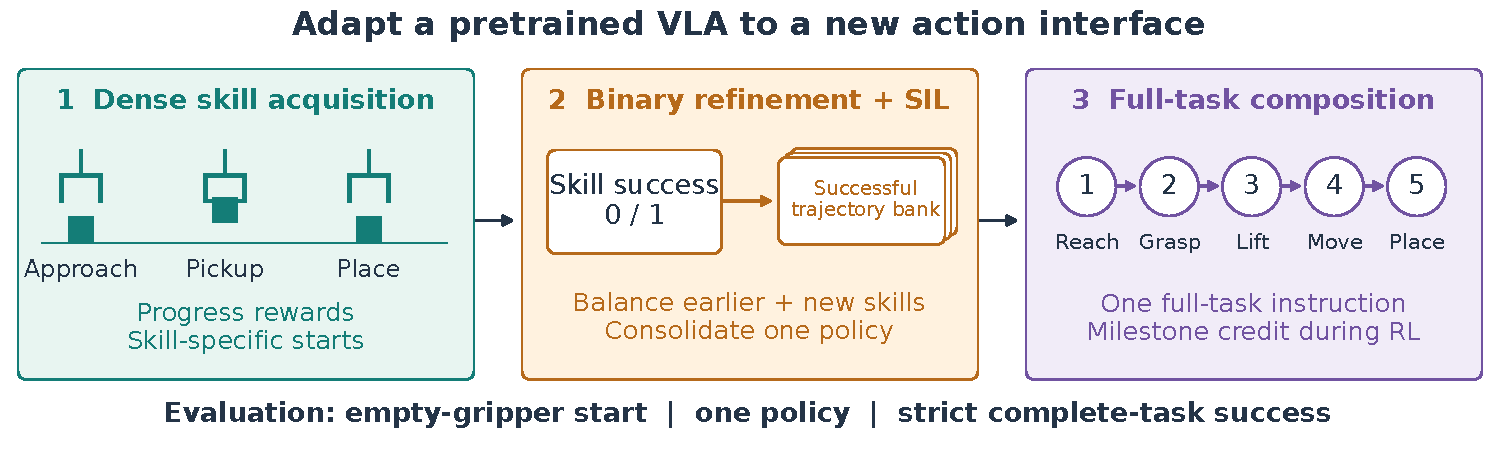
\includegraphics[width=\textwidth]{figures/pipeline_overview.pdf}
\captionof{figure}{Proposed pipeline. Dense feedback acquires skills; binary refinement and balanced self-imitation consolidate them; milestone-based RL learns the complete task under one instruction. Skill-specific resets are used during acquisition. Full-task evaluation starts with an empty gripper and uses no external switching between specialists.}
\label{fig:hero}
\end{minipage}
\vspace{1em}}
\maketitle
\begin{center}\small\textbf{WORKING VISUAL DRAFT --- 26 October 2026}\end{center}
\begin{abstract}
Adapting a vision-language-action (VLA) model to a new robot is difficult when its action interface produces few successful rollouts. We propose a three-stage reinforcement learning pipeline: dense skill acquisition, binary refinement with self-imitation, and milestone-based full-task composition. Dense rewards guide early exploration. A balanced bank of successful trajectories helps recover earlier skills, and milestone credit trains one policy to execute the complete instruction. We implement the pipeline with pretrained SmolVLA, LoRA, and an embodiment-specific residual controller. The controller achieves 61.43\% strict pick-and-place success on CDPR simulation development scenes. A retention experiment increases reaching success from 8.0\% to 31.1\% while preserving placement performance. On LIBERO-Spatial, phase-aware dense feedback reaches 65.3\% success versus 61.7\% with terminal-only reward. These results support structured feedback and skill consolidation; controlled ablations of the complete schedule remain open.
\end{abstract}

\begin{IEEEkeywords}
Robot learning, reinforcement learning, manipulation, vision-language-action models, robot adaptation.
\end{IEEEkeywords}
\section{Introduction}\label{sec:introduction}
Vision-language-action (VLA) models provide useful visual and language representations for robot control. A new embodiment can still require a different action mapping. Before this mapping is learned, complete-task success may be too rare to provide a useful binary learning signal.

Consider ``put the apple on the plate.'' The robot must approach, grasp, lift, transport, and release the object. Terminal failure alone does not distinguish a missed grasp from a failed release. Learning these skills separately improves the starting point, but training a new skill can also erase earlier behavior. The final policy must both retain the skills and connect them under one instruction.

We address these problems with the pipeline in Fig.~\ref{fig:hero}. Dense rewards first guide individual skill learning. Binary rewards then target skill completion, and balanced self-imitation consolidates successful experience across instructions. Finally, milestone-based RL trains complete-task execution from ordinary empty-gripper starts.

We study embodiment adaptation with SmolVLA on a cable-driven parallel robot (CDPR). A learned residual controller adapts a retained pretrained action expert to the target interface. We also study reward construction with OpenVLA-OFT on LIBERO, where an established action policy lets us examine intermediate feedback separately from learning a new interface.

Our contributions are (i) a staged skill-learning and composition pipeline, (ii) a residual implementation with explicit milestone credit, and (iii) empirical evidence on skill recovery, full-task execution, and phase-aware feedback. LIBERO evaluates reward design; it does not evaluate the complete adaptation schedule.

\section{Related Work}\label{sec:related}
\textbf{Group-relative RL and dynamic sampling.} GRPO estimates policy advantages by comparing returns within groups of sampled trajectories~\cite{deepseekmath}. DAPO introduces dynamic sampling that filters groups with uniform binary outcomes and collects additional samples to maintain an informative training batch~\cite{dapo}. SimpleVLA-RL adapts group-relative optimization to interactive robot rollouts, using dynamic sampling and exploration enhancements to improve task execution and discover behaviors beyond the supervised demonstrations~\cite{simplevlarl}. These methods provide a basis for learning task-specific behavior through interaction. We use DAPO-style group filtering and resampling during skill learning.

\textbf{Alternating RL and supervised learning.} iRe-VLA alternates online RL on a lightweight action head with a frozen vision-language backbone and supervised updates using expert data together with successful online trajectories~\cite{irevla}. This separates exploration from supervised consolidation while allowing the large model to benefit from collected experience. Our self-imitation step fits an instruction-balanced mixture of earlier and current successes to retain skills during sequential training.

\textbf{Residual RL and distillation.} Probe, Learn, Distill (PLD) trains lightweight residual specialists over a frozen VLA, collects trajectories through policy-aligned residual interventions, and distills the resulting data into the generalist~\cite{pld}. We adopt the residual-learning principle to adapt the target action interface. Our training procedure links skill acquisition and successful-experience consolidation before learning to execute the complete instruction.

Our earlier work studied RL bootstrapping of OpenVLA-OFT on the CDPR for directional motion and object reaching~\cite{nurtdinov2026rlboot}. The present work extends the study to complete pick-and-place through skill consolidation and milestone-based learning with a SmolVLA residual controller.

\section{Problem Formulation}\label{sec:problem}
A policy receives camera images, proprioception, and instruction $\ell$, and predicts an action chunk. The controller executes a prefix before replanning. Let $h_t$ denote the available observation history and $c$ the scene initialization. We optimize binary complete-task success $Y(\tau)$:
\begin{equation}
J(\theta)=\mathbb E_{(c,\ell)\sim\rho_{\rm full},\,\tau\sim P_\theta(\cdot\mid c,\ell)}[Y(\tau)].
\end{equation}
Individual skills have their own instructions, success predicates, and reset distributions $\rho_k$. Placement from a held-object start is therefore a skill test, not full pick-and-place. A training stage is a step in the learning schedule; a task phase is progress within an episode.

The CDPR action has five channels: Cartesian translation, yaw, and gripper control. Strict success requires grasp, held lift, intentional release, and native placement, without carry-slip or wrong-placement events. LIBERO uses its native goal verifier~\cite{libero}. We report these different evaluation settings separately.

\section{Methods}\label{sec:method}
\section{Problem Formulation}\label{sec:problem}
A policy receives camera images, proprioception, and instruction $\ell$, and predicts an action chunk. The controller executes a prefix before replanning. Let $h_t$ denote the available observation history and $c$ the scene initialization. We optimize binary complete-task success $Y(\tau)$:
\begin{equation}
J(\theta)=\mathbb E_{(c,\ell)\sim\rho_{\rm full},\,\tau\sim P_\theta(\cdot\mid c,\ell)}[Y(\tau)].
\end{equation}
Individual skills have their own instructions, success predicates, and reset distributions $\rho_k$. Placement from a held-object start is therefore a skill test, not full pick-and-place. A training stage is a step in the learning schedule; a task phase is progress within an episode.

The CDPR action has five channels: Cartesian translation, yaw, and gripper control. Strict success requires grasp, held lift, intentional release, and native placement, without carry-slip or wrong-placement events. LIBERO uses its native goal verifier~\cite{libero}. We report these different evaluation settings separately.


\subsection{Dense Acquisition, Binary Refinement, and Self-Imitation}
We first train approach, pickup, and placement skills with dense rewards. Distance reduction and manipulation events guide exploration before skill success becomes common. After dense acquisition, we refine the skills using binary success rewards.

Successful trajectories are retained by instruction. When later training degrades earlier skills, self-imitation fits a balanced mixture of earlier and current successes:
\begin{equation}
\mathcal L_{\rm SI}=\mathbb E_{\rm success}
\left[\|\hat a-a\|^2\right].
\label{eq:si_loss}
\end{equation}
Here $\hat a$ is the predicted action and $a$ is the recorded executed action. The average balances instructions and excludes unused action slots. Policy-dependent features are refreshed before fitting. Balancing matters because imitating only the newest skill can reinforce forgetting.

Algorithm~\ref{alg:paper_pipeline} summarizes the schedule. Progress is checked with fixed skill evaluations. After an initial training period, automated stages can end at a success target or a plateau; budget exhaustion also ends a stage. The CDPR sequence used validation-guided manual transitions. After consolidation, all learned skills are evaluated again. Automated runs retain the consolidation update only when recovery improves the degraded skills on average and keeps other skills within tolerance.
% Method-level schedule. Automatic stopping is implemented for WX200;
% the historical CDPR sequence used validation-guided manual transitions.
\begin{algorithm}[!t]
\caption{Staged VLA adaptation}
\label{alg:paper_pipeline}
\small
\begin{algorithmic}[1]
\Require Pretrained VLA, skill instructions, fixed evaluations
\State Initialize the target action controller and success banks
\For{reward mode: dense acquisition, then binary refinement}
    \For{skill: approach, pickup, placement}
        \Repeat
            \State Collect same-scene rollout groups for the skill
            \State Update with $\mathcal L_{\rm RL}$; retain successful trajectories
            \State Evaluate skill success
        \Until{target, plateau, or stage budget ends training}
        \State Evaluate retention of all learned skills
        \If{earlier skills have degraded}
            \State Balance earlier and current successful experience
            \State Fit $\mathcal L_{\rm SI}$; validate recovery and retention
        \EndIf
    \EndFor
\EndFor
\Repeat
    \State Collect full-task rollouts from empty-gripper starts
    \State Assign milestone credit; protect achieved prefix skills
    \State Update with $\mathcal L_{\rm RL}$; evaluate complete-task success
\Until{target, plateau, or full-task budget ends training}
\State \Return One policy for the complete instruction
\end{algorithmic}
\end{algorithm}


\subsection{SmolVLA with an Embodiment-Specific Residual}
Figure~\ref{fig:architecture} shows one implementation of the pipeline. The pretrained SmolVLA expert supplies an action prior, mapped to the target control interface. In our five-channel controller, eight action slots give
\begin{equation}
p\in\mathbb R^{40}
\qquad
(8\text{ slots}\times5\text{ channels}).
\label{eq:prior}
\end{equation}
A frozen visual projection supplies 512 features; six proprioceptive values complete the 518-dimensional observation. The residual receives this observation and the 40-dimensional prior, and predicts a bounded correction. The combined action is bounded before execution.

LoRA adapts the action expert during earlier training. In the evaluated full-task continuation, the inherited VLA and LoRA weights are frozen while the residual and exploration parameters are trained. The backbone, action mapping, and feature dimensions can change with the embodiment; the training schedule remains the same.

\begin{figure*}[!t]
\centering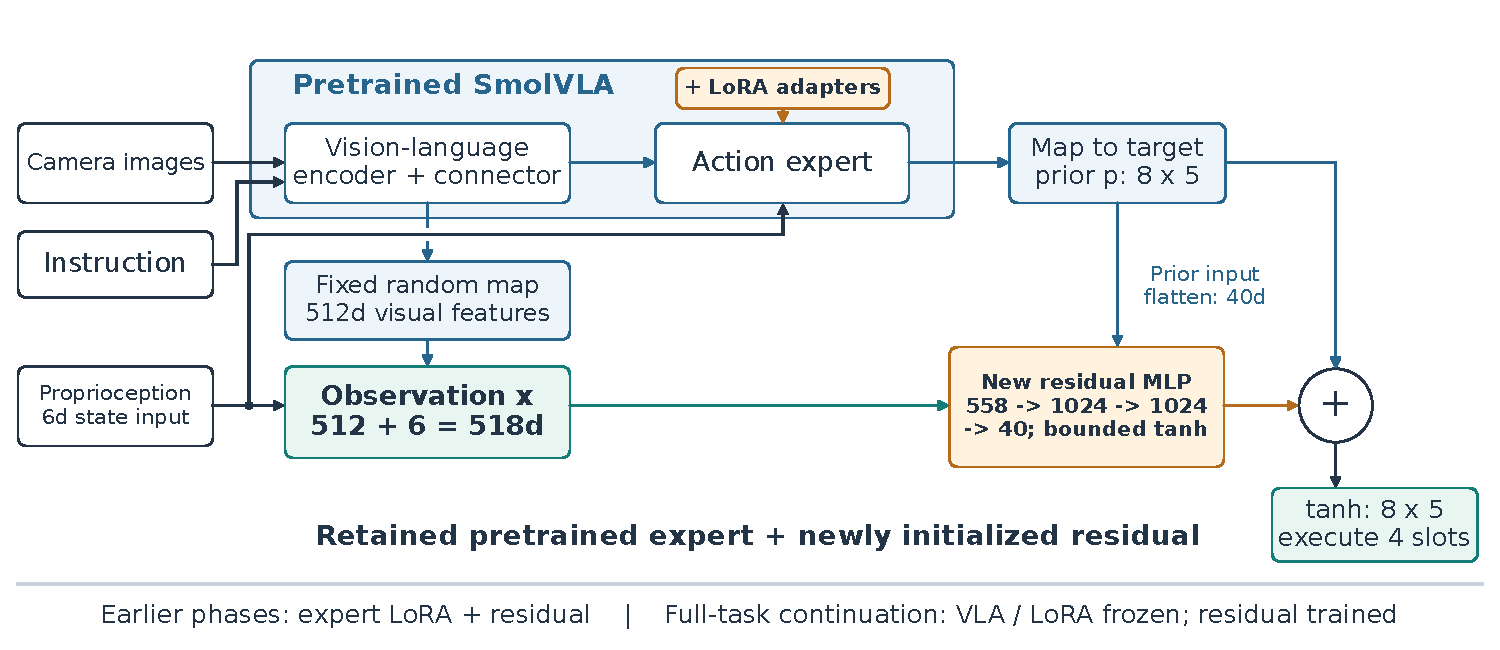
\includegraphics[width=\textwidth]{figures/smolvla_residual_lora.pdf}
\caption{SmolVLA implementation of the pipeline. The added residual combines 518 observation features with a 40-dimensional action prior. LoRA adapts the pretrained expert during earlier training; the evaluated full-task continuation freezes the VLA and LoRA weights. Feature and action dimensions refer to the five-channel controller.}
\label{fig:architecture}
\end{figure*}

\subsection{Milestone-Based Full-Task Composition}
After skill consolidation, one policy learns the complete instruction from empty-gripper starts. No external controller switches between specialist policies. Approach, held pickup, and final placement serve as milestones for assigning credit within a rollout.

The main rule is simple: a later placement failure should not remove the local credit for a successful approach or pickup. We compare milestone outcomes within groups of rollouts from the same scene. Actions receive credit for the milestone they contribute to, while full-task success provides an additional preference for completing the chain. A negative completion bonus is suppressed on already achieved approach and pickup milestones. Placement receives its completion credit once (Fig.~\ref{fig:credit}).

This rule preserves useful partial behavior while training the remaining task. It controls the assigned credit; it does not prevent interference through shared network parameters.

\begin{figure}[!t]
\centering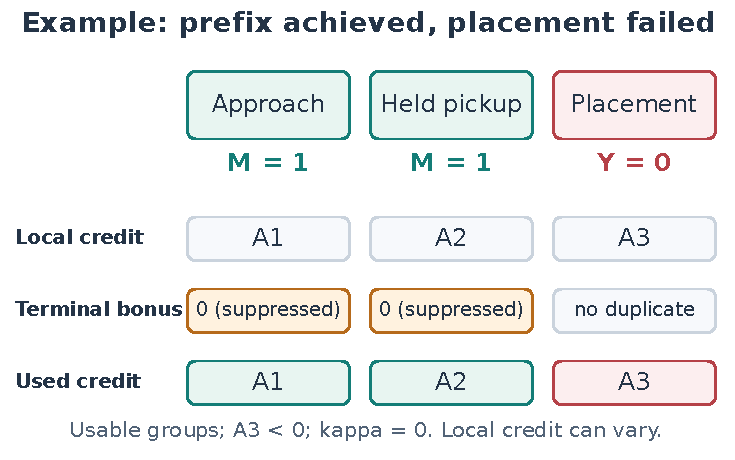
\includegraphics[width=\columnwidth]{figures/milestone_credit.pdf}
\caption{Credit assignment when approach and pickup succeed but placement fails. Local credit remains available for the achieved skills. The negative completion bonus is blocked on these skills, while placement is trained from its own outcome. The diagram assumes groups with informative milestone comparisons.}
\label{fig:credit}
\end{figure}

\subsection{Stabilized Policy Updates}\label{sec:rl_loss}
We use a clipped group-relative policy loss with entropy regularization:
\begin{equation}
\mathcal L_{\rm RL}=\mathcal L_{\rm clip}-\eta\mathcal H.
\label{eq:rl_loss}
\end{equation}
The clipped loss compares rollouts within each scene group and limits the incentive for large changes in action likelihood. We use separate upper and lower clipping bounds. The entropy term $\mathcal H$, weighted by $\eta$, maintains exploration during manipulation and composition. Together, these choices help keep early updates conservative while successful behavior is still rare.

For bounded continuous actions, likelihoods are computed from the sampled Gaussian commands before clipping, while the robot executes the clipped commands. This keeps the loss consistent with the sampling process at action limits~\cite{capg}. Self-imitation uses the simpler regression loss in Eq.~\eqref{eq:si_loss}.

\label{sec:dense_method}
To examine intermediate feedback on a standard benchmark, the LIBERO experiment compares terminal-only, phase-only, and combined dense-and-phase rewards. The combined reward uses a manually defined sequence of reach, grasp, lift, move, and place phases, with a hand-specified progress function for each phase.

At each simulator step, the tracker uses object and gripper state to compute progress for the active phase. Reaching progress increases as gripper--object distance decreases; grasping combines proximity with gripper closure and grasp state; lifting uses height gained above the initial object position; transport uses planar object--target distance; placement uses target proximity, release, and environment success. Each progress measure is normalized to the interval from zero to one. For progress $p_t$ and the phase's previous maximum $p_{\rm best}$, the rewarded increment is $\max(p_t-p_{\rm best},0)$. A completion predicate advances the tracker to the next phase and produces a phase bonus. The weighted progress increment and phase bonus are bounded and combined with terminal feedback. The native task-success verifier remains unchanged.

In the phase-only condition, the continuous progress weight is zero, leaving phase-completion bonuses and terminal feedback.

The dense construction requires a progress function, normalization, and relevant state variables for every phase. Extending it to a new multi-stage task therefore requires further task-specific reward design. This motivates our use of dense feedback for initial skill acquisition and binary milestones for composition: the latter require completion predicates without a continuous progress function for every part of the instruction.

\section{Why Intermediate Feedback Helps}\label{sec:theory}
For $G$ independent candidates from one scene, each with binary success probability $p$, the probability of a mixed-outcome group is
\begin{equation}
P_{\rm mixed}=1-p^G-(1-p)^G.
\label{eq:mixed}
\end{equation}
At $G=8$, it is 21.6\% for $p=0.03$ and 94.2\% for $p=0.30$. Milestones can therefore provide contrast before full success becomes common. Dense progress can distinguish candidates within one milestone level. Neither guarantees useful learning if the feedback is constant or the collector rejects the group.

With separate Bernoulli gates and raw on-policy ascent, suppressing negative completion credit on achieved gates makes each gate's update nonnegative. This finite-model property does not extend directly to a shared neural controller, PPO clipping, or optimizer momentum. We use it to explain the credit rule, without claiming monotonic improvement~\cite{trpo}.


\section{Why Intermediate Feedback Helps}\label{sec:theory}
For $G$ independent candidates from one scene, each with binary success probability $p$, the probability of a mixed-outcome group is
\begin{equation}
P_{\rm mixed}=1-p^G-(1-p)^G.
\label{eq:mixed}
\end{equation}
At $G=8$, it is 21.6\% for $p=0.03$ and 94.2\% for $p=0.30$. Milestones can therefore provide contrast before full success becomes common. Dense progress can distinguish candidates within one milestone level. Neither guarantees useful learning if the feedback is constant or the collector rejects the group.

With separate Bernoulli gates and raw on-policy ascent, suppressing negative completion credit on achieved gates makes each gate's update nonnegative. This finite-model property does not extend directly to a shared neural controller, PPO clipping, or optimizer momentum. We use it to explain the credit rule, without claiming monotonic improvement~\cite{trpo}.

\section{Experiments}\label{sec:experiments}
We evaluate three aspects of the approach: full-task composition, retention during sequential learning, and intermediate feedback. SmolVLA experiments test the adaptation pipeline in CDPR simulation. OpenVLA-OFT experiments test reward design on the ten LIBERO-Spatial tasks. The ongoing WX200 study examines another embodiment.

\subsection{SmolVLA: Complete-Task Adaptation}\label{sec:cdpr_results}
The CDPR simulation uses MuJoCo Warp/MJ-Lab, four object categories (apple, orange, potato, and tomato), and plate or bowl destinations. The action interface controls Cartesian translation, yaw, and the gripper. Strict success requires grasp, held lift, intentional release, and correct placement, without carry slip or wrong-placement events.

Separate evaluation covers 512 development scenes with four repeats each, excluding the in-run validation panel. Each attempt starts with an empty gripper and uses one full-task instruction, without teacher assistance. A later continuation supplies only TensorBoard in-run validation, with 1,024 attempts per reading. These two protocols are reported separately. All attempts, including numerical failures, remain in their respective denominators.
\subsection{Complete-Task Execution}
The adapted SmolVLA controller completes 1,258 of 2,048 attempts (61.43\%) from empty-gripper starts. Table~\ref{tab:cdpr} reports its task outcomes. Held lift occurs in 85.89\% of attempts, but only 71.52\% of held-lift attempts reach strict completion. Transport and release remain a major bottleneck. Plate and bowl completion rates are 68.58\% and 54.22\%, respectively. These are development results from one training lineage.
\begin{table}[t]
\caption{CDPR complete-task results at the 60.03M-action endpoint. Rates use all 1,024 attempts: 512 plate and 512 bowl episodes. Event flags can overlap.}
\label{tab:cdpr}\centering\small
\begin{tabular}{@{}lr@{}}\toprule
Outcome & Attempts (\%)\\\midrule
Physical grasp & 92.48\\
Held lift & 88.28\\
Strict completion (723/1,024) & 70.61\\
Carry slip & 16.70\\
Wrong placement & 14.16\\
Numerical failure & 0.88\\\bottomrule
\end{tabular}
\end{table}


\subsection{Base-Policy Skill Learning and Retention}\label{sec:skill_retention}
These measurements concern dense-reward training of simple CDPR skills and their consolidation into a base policy, before full-task composition. Each skill uses the instruction and reset protocol in Section~\ref{sec:skill_acquisition}; placement tests start with the object already held. Learning a new skill can degrade previously learned behavior, although the same policy must retain all component skills to execute the complete multi-stage task.

\begin{figure*}[!t]
\centering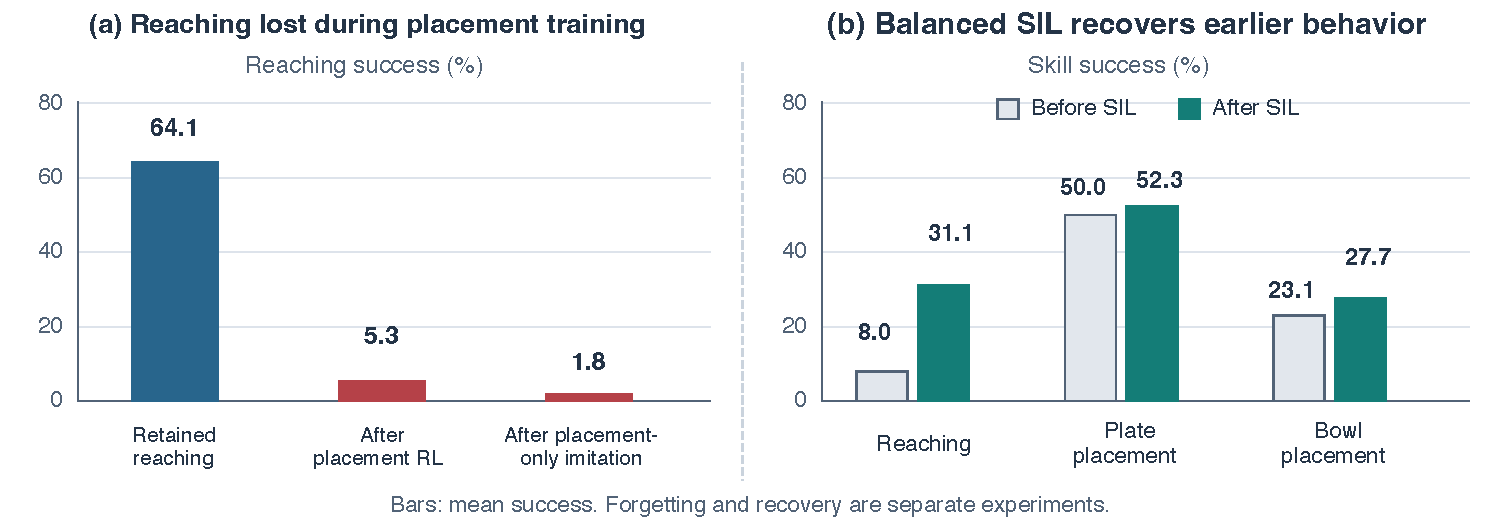
\includegraphics[width=\textwidth]{figures/skill_retention.pdf}
\caption{Base-policy skill recovery before full-task composition. Bars show means and points show individual evaluation rounds: three for reaching and two for each placement skill, per condition. Reaching uses the instruction \emph{move to \textless object\textgreater}; placement starts with the object already held. Reaching partially recovers while both placement means increase.}
\label{fig:retention}
\end{figure*}

In a forgetting evaluation, mean reaching success falls from 64.1\% for the reaching reference to 5.3\% after placement RL, over three evaluation rounds per condition. The recovery evaluation in Fig.~\ref{fig:retention} is a separate measurement: balanced self-imitation raises reaching success from 8.0\% to 31.1\%. Plate placement changes from 50.0\% to 52.3\%, and bowl placement from 23.05\% to 27.65\%. The bank combines earlier reaching successes with current placement successes, balancing the retained data by instruction.

Recovery is partial, with placement performance retained while reaching improves. Table~\ref{tab:skill_matrix} summarizes skill-specific RL references and a shared policy after subsequent consolidation. Evaluation reset distributions differ across stages. The shared policy succeeds on all four skills, although pickup remains weak. These skill evaluations do not isolate the contribution of self-imitation to final full-task success.

% Reaching reference: evidence/skill_retention_rounds.json, forgetting comparison.
% Other rows: ../CDPR_CONSOLIDATED_PROGRESS_REPORT.md, instruction success table;
% consolidation is the Cycle 3 shared policy, evaluated before composition.
\begin{table}[!ht]
\caption{Skill success (\%) by training stage. Placement starts with the object held; --- denotes an unreported result.}
\label{tab:skill_matrix}\centering\small
\begin{tabular}{@{}lrrrr@{}}\toprule
Training stage & Reach & Pickup & Plate & Bowl\\\midrule
Reaching RL & 64.1 & --- & --- & ---\\
Pickup RL & --- & 26.0 & --- & ---\\
Placement RL & --- & --- & 71.0 & 32.0\\
After consolidation & 47.8 & 11.9 & 73.8 & 53.5\\\bottomrule
\end{tabular}
\end{table}



\subsection{Intermediate Feedback on LIBERO-Spatial}\label{sec:libero_results}
This experiment compares feedback for complete manipulation instructions, using OpenVLA-OFT and SimpleVLA-RL to hold the backbone and training framework fixed across reward conditions~\cite{openvlaoft,simplevlarl}. It tests an ingredient of the adaptation pipeline; the complete training schedule is evaluated on the CDPR.

We fine-tune with LoRA on the ten LIBERO-Spatial tasks~\cite{libero}, using the feedback variants in Section~\ref{sec:composition}. All runs share a 61.0\% initialization and use 300 validation rollouts per endpoint. The terminal-only baseline is trained with SimpleVLA-RL under the same 160-update budget and terminal verifier coefficient 5 as the dense-and-phase condition. The phase-only condition uses phase-completion bonuses with terminal verifier coefficient 1 and a 110-update budget.

At 160 updates, dense feedback reaches 65.3\% success versus 61.7\% with terminal-only reward, a difference of 3.6 percentage points. Filtered dense feedback reaches 64.7\% at 50 updates.
\begin{table}[t]
\caption{LIBERO reward comparison and low-success task. Success and $\Delta$ are percentages and percentage points. Aggregate endpoints use 300 validation rollouts; final task\_1 denominators are unreported. Different update budgets are shown explicitly.}
\label{tab:libero}\centering\small
\begin{tabular}{@{}lrrr@{}}\toprule
Configuration & Updates & Success & $\Delta$\\\midrule
\multicolumn{4}{@{}l}{LIBERO-Spatial: initial 61.0\%}\\
Terminal only, $\lambda=5$ & 160 & 61.7 & +0.7\\
Dense, $\lambda=5$ & 160 & 65.3 & +4.3\\
Filtered dense, $\lambda=5$ & 50 & 64.7 & +3.7\\
Dense, $\lambda=1$ & 110 & 61.0 & +0.0\\
Phase only, $\lambda=1$ & 110 & 62.3 & +1.3\\
\midrule
\multicolumn{4}{@{}l}{task\_1: initial 2.0\% (1,000 rollouts)}\\
Terminal only & 20 & 11.0 & +9.0\\
Dense & 20 & 18.0 & +16.0\\
\bottomrule
\end{tabular}
\end{table}


With the lower terminal reward weight, phase-only and dense feedback reach 62.3\% and 61.0\%, respectively. Their phase weights also differ, so this comparison does not isolate within-phase progress. On the low-success task, dense and terminal-only training reach 18\% and 11\% after 20 updates, from the same 2\% initialization.

The matched-budget comparisons support intermediate feedback in these settings. Different budgets across the other conditions prevent a general efficiency claim.

\subsection{Reserved Robot Illustrations}\label{sec:hardware_results}
The WX200 layout in Fig.~\ref{fig:wx200} reserves the apparatus, control axes, and a time-ordered task sequence. Actual images and measurements will replace these slots. No hardware result is reported in this draft.

\begin{figure*}[!t]
\centering
\IfFileExists{figures/wx200/panel.pdf}{\includegraphics[width=\textwidth]{figures/wx200/panel.pdf}}{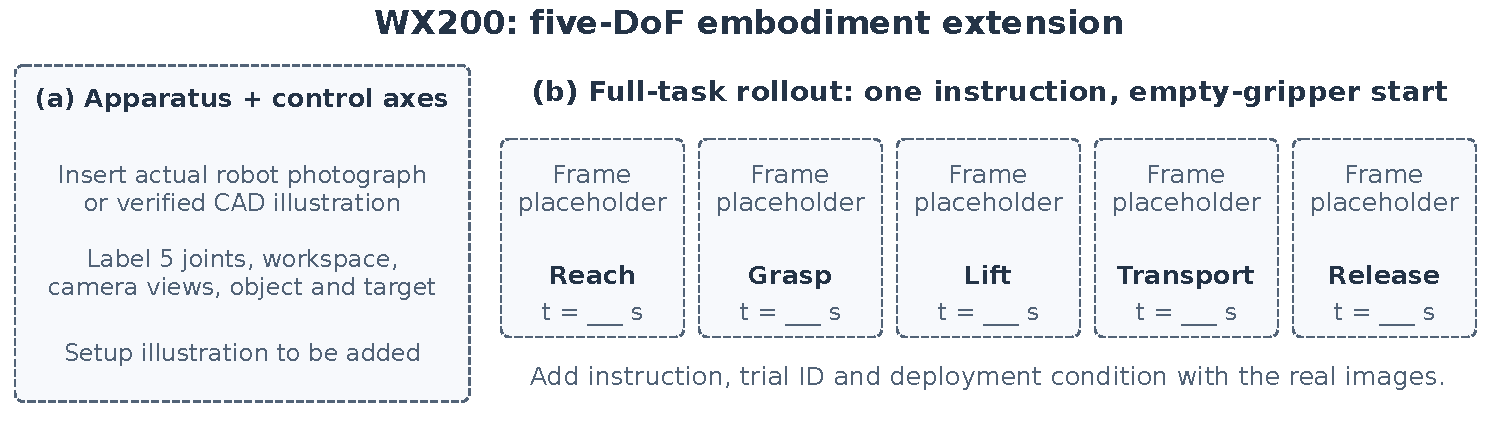
\includegraphics[width=\textwidth]{figures/wx200_slots.pdf}}
\caption{Reserved WX200 illustrations. (a) Five-DoF robot, workspace, cameras, and control-axis annotation. (b) Actual rollout frames for reach, grasp, lift, transport, and release. Add timestamps and the task instruction. The current panels are layout placeholders and contain no experimental evidence.}
\label{fig:wx200}
\end{figure*}

\subsection{Scope of the Evidence}
The complete-task result comes from one SmolVLA training lineage. The retention results summarize a small number of rounds, and the LIBERO results are descriptive endpoint comparisons. Neither study isolates every stage of the pipeline. Earlier assisted training is part of the inherited CDPR policy; the reported full-task evaluation uses no assistance.


% Results are integrated into Experiments in sections/05_experimental_setup.tex.
% This file is retained as a pointer for earlier integration notes.

\subsection{Scope of the Evidence}
The complete-task result comes from one SmolVLA training lineage. The retention results summarize a small number of rounds, and the LIBERO results are descriptive endpoint comparisons. Neither study isolates every stage of the pipeline. Earlier assisted training is part of the inherited CDPR policy; the reported full-task evaluation uses no assistance.

\section{Conclusion}\label{sec:conclusion}
We presented dense skill acquisition, binary refinement with self-imitation, and milestone-based full-task composition for VLA adaptation. A SmolVLA residual controller achieves 61.43\% strict CDPR development success. Balanced consolidation partially recovers an earlier skill, and LIBERO experiments show an observed benefit of phase-aware feedback. Further controlled experiments are needed to establish the contribution of each training stage.

\IEEEtriggeratref{9}
\bibliographystyle{IEEEtran}
\bibliography{references}
\end{document}
